\documentclass[tikz,border=5pt]{standalone}
\usepackage{tikz}
\usetikzlibrary{arrows.meta}

% Atlas color palette
\definecolor{AtlasTeal}{HTML}{5BA4A4}
\definecolor{AtlasWarm}{HTML}{C17F59}
\definecolor{AtlasSage}{HTML}{7A9E7E}
\definecolor{AtlasTealLight}{HTML}{D4E8E8}

\begin{document}
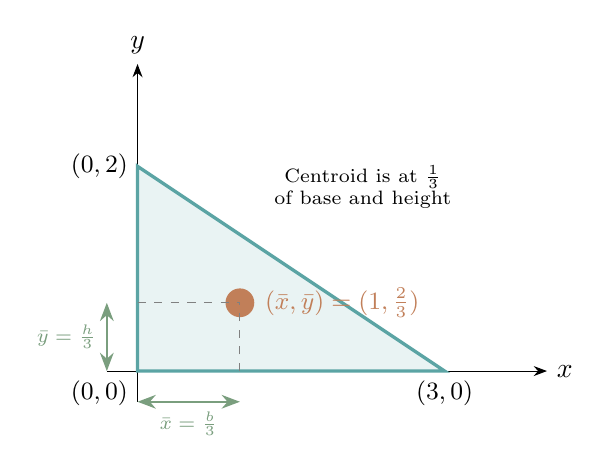
\begin{tikzpicture}[>=Stealth, scale=1.3]
    % Axes
    \draw[->] (-0.3,0) -- (4,0) node[right] {$x$};
    \draw[->] (0,-0.3) -- (0,3) node[above] {$y$};
    
    % Region: triangle with vertices (0,0), (3,0), (0,2)
    \fill[AtlasTealLight, opacity=0.5] (0,0) -- (3,0) -- (0,2) -- cycle;
    \draw[AtlasTeal, very thick] (0,0) -- (3,0) -- (0,2) -- cycle;
    
    % Centroid marker
    \fill[AtlasWarm] (1, 0.667) circle (4pt);
    \node[AtlasWarm, right, font=\small] at (1.15, 0.667) {$(\bar{x}, \bar{y}) = (1, \frac{2}{3})$};
    
    % Vertices labels
    \node[below left, font=\small] at (0,0) {$(0,0)$};
    \node[below, font=\small] at (3,0) {$(3,0)$};
    \node[left, font=\small] at (0,2) {$(0,2)$};
    
    % Dashed lines to centroid
    \draw[dashed, gray] (1, 0) -- (1, 0.667);
    \draw[dashed, gray] (0, 0.667) -- (1, 0.667);
    
    % Distance markers
    \draw[<->, AtlasSage, thick] (0, -0.3) -- node[below, font=\scriptsize] {$\bar{x} = \frac{b}{3}$} (1, -0.3);
    \draw[<->, AtlasSage, thick] (-0.3, 0) -- node[left, font=\scriptsize] {$\bar{y} = \frac{h}{3}$} (-0.3, 0.667);
    
    % Annotation
    \node[font=\scriptsize, text width=2.5cm, align=center] at (2.2, 1.8) 
        {Centroid is at $\frac{1}{3}$ of base and height};
\end{tikzpicture}
\end{document}
